

\begin{figure}[th]
	\centering
	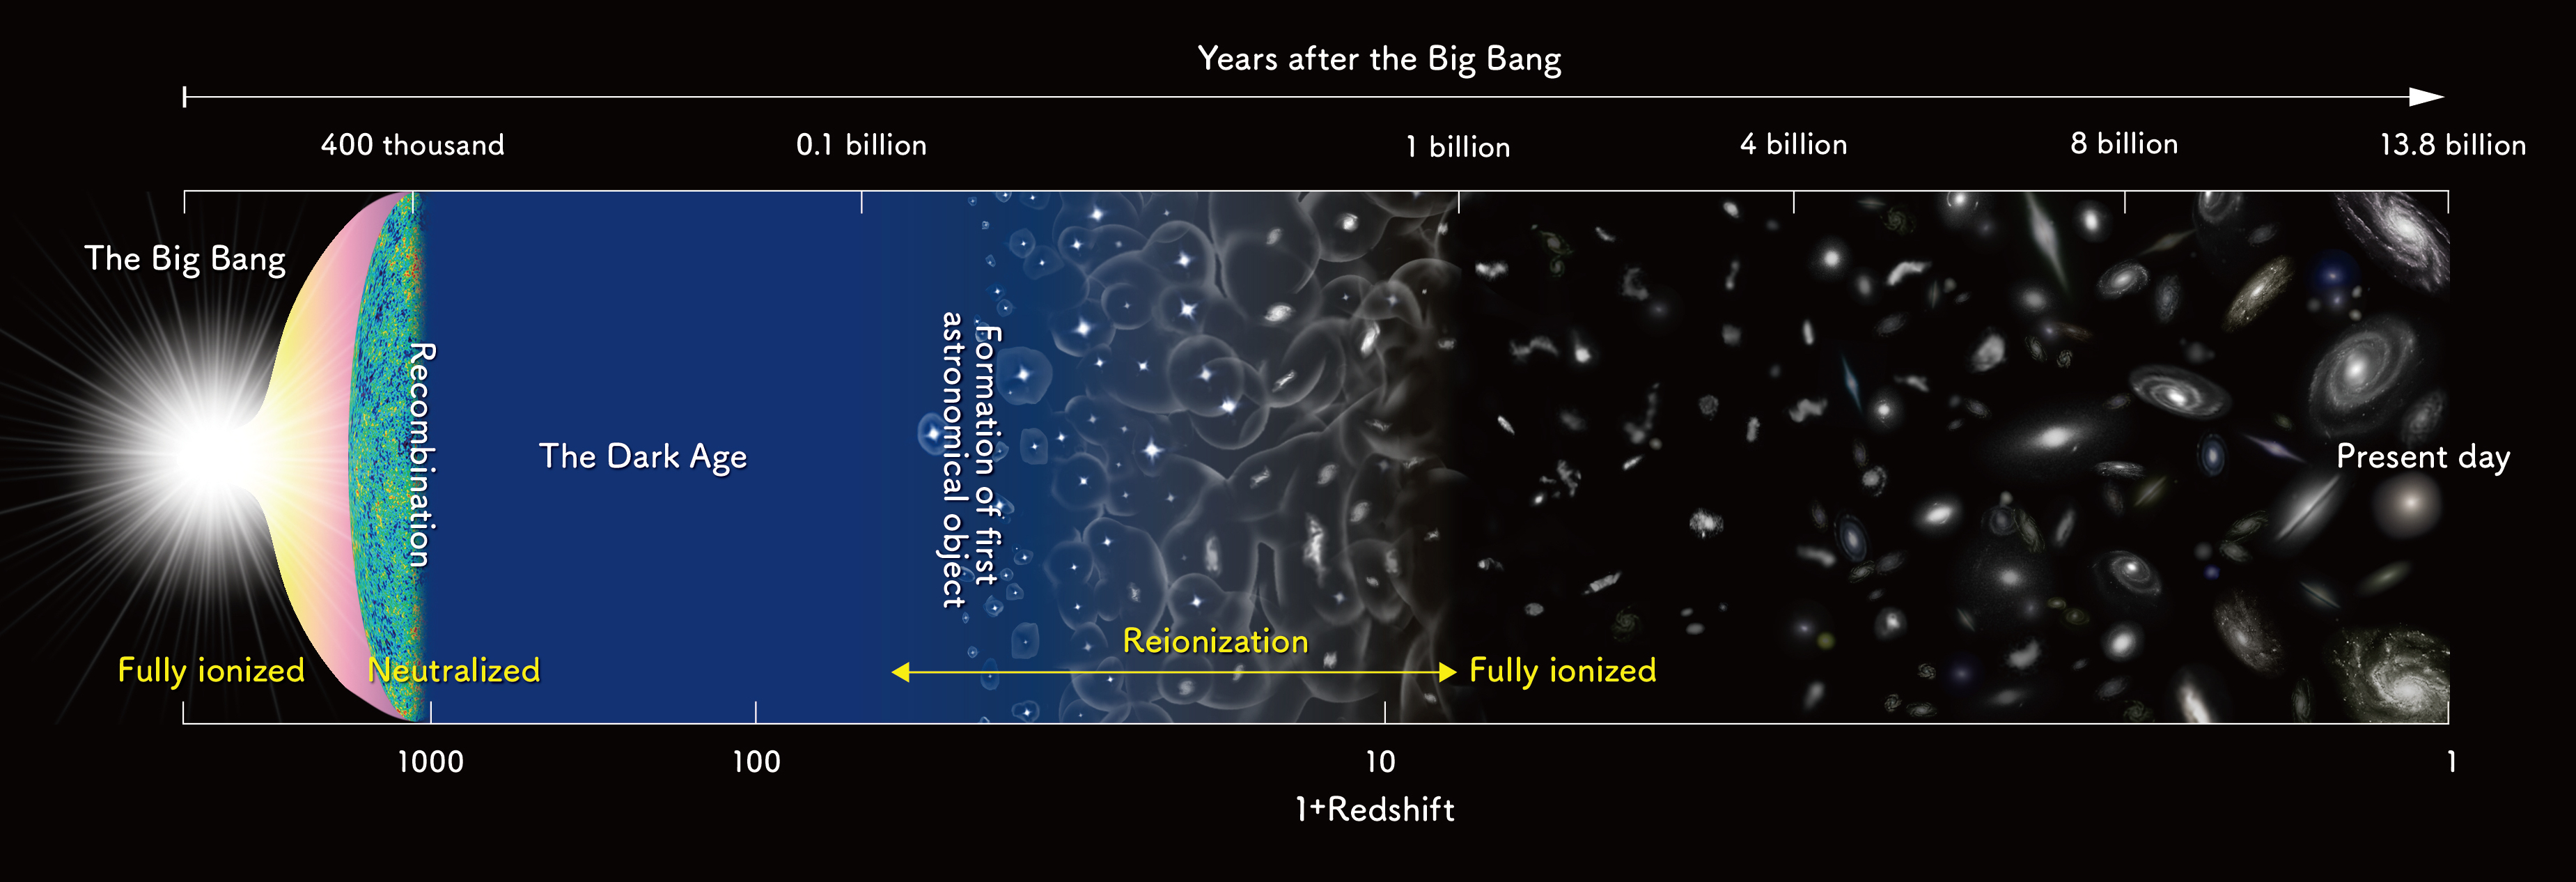
\includegraphics[width=1.0\textwidth]{intro/reionization.png}
	\caption[Epoch of Reionization Timeline]{Timeline of the history of the universe from its formation (left) to present day (right).}
	\label{fig:timeline}
\end{figure}



\begin{figure}[th]
	\centering
	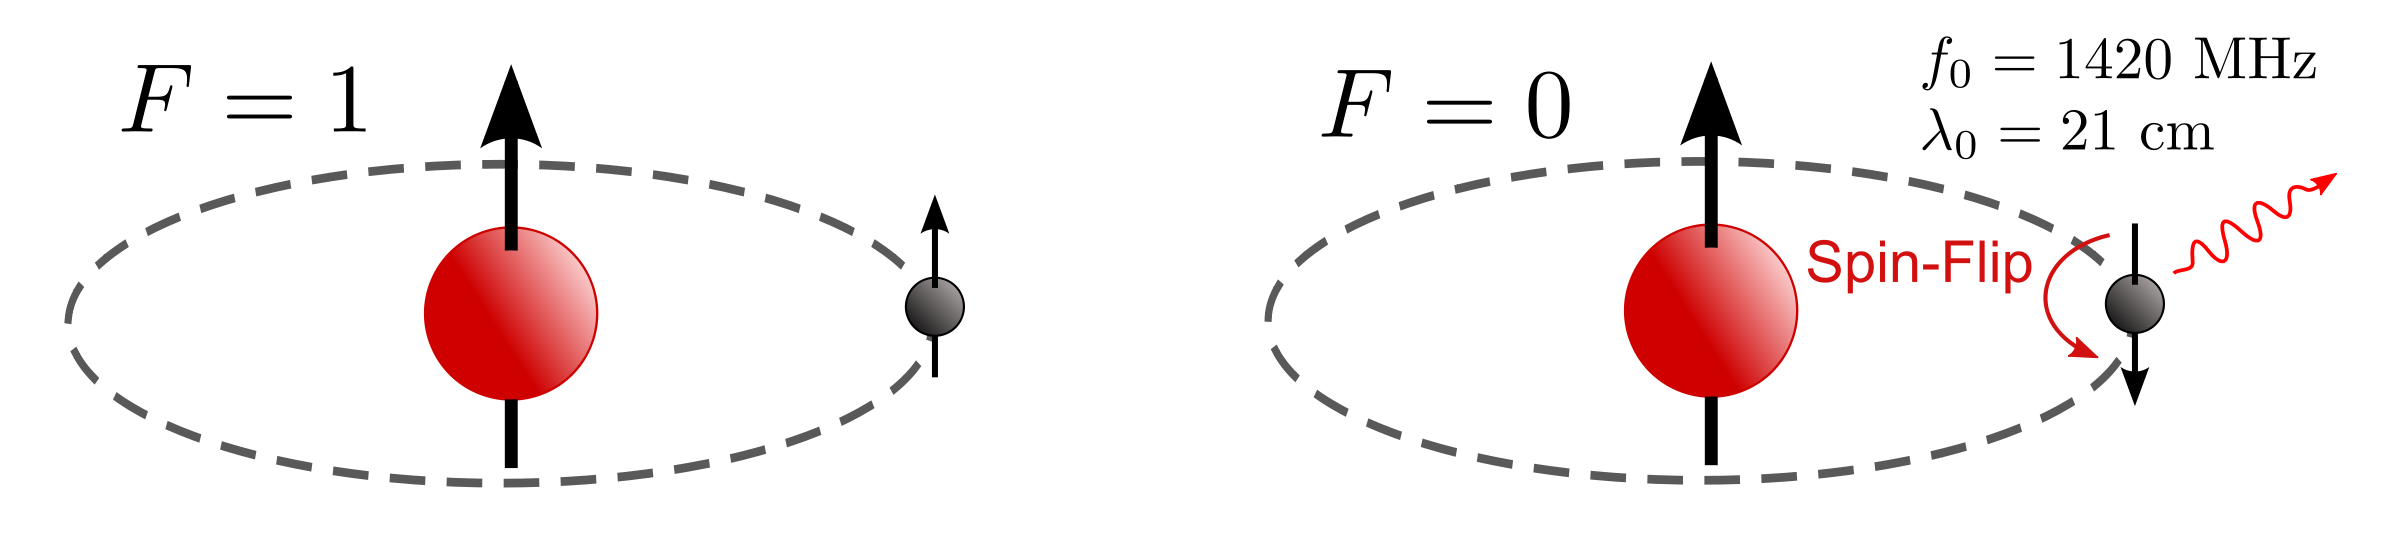
\includegraphics[width=0.90\textwidth]{spin_flip_H.png}
	\caption[Spin-Flip Transition of Neutral Hydrogen]{A depiction of the spin-flip transition of neutral hydrogen. Initially,
																					 the spin of the proton and electron are parallel and oriented
																					 in the same direction. The transition occurs when the electron's spin spontaneously
																					 flips from the higher energy parallel alignment to the lower energy anti-parallel alignment,
																					 releasing a photon with a wavelength of 21\,cm.}
	\label{fig:spin_flip}
\end{figure}

\begin{figure}[th]
	\centering
	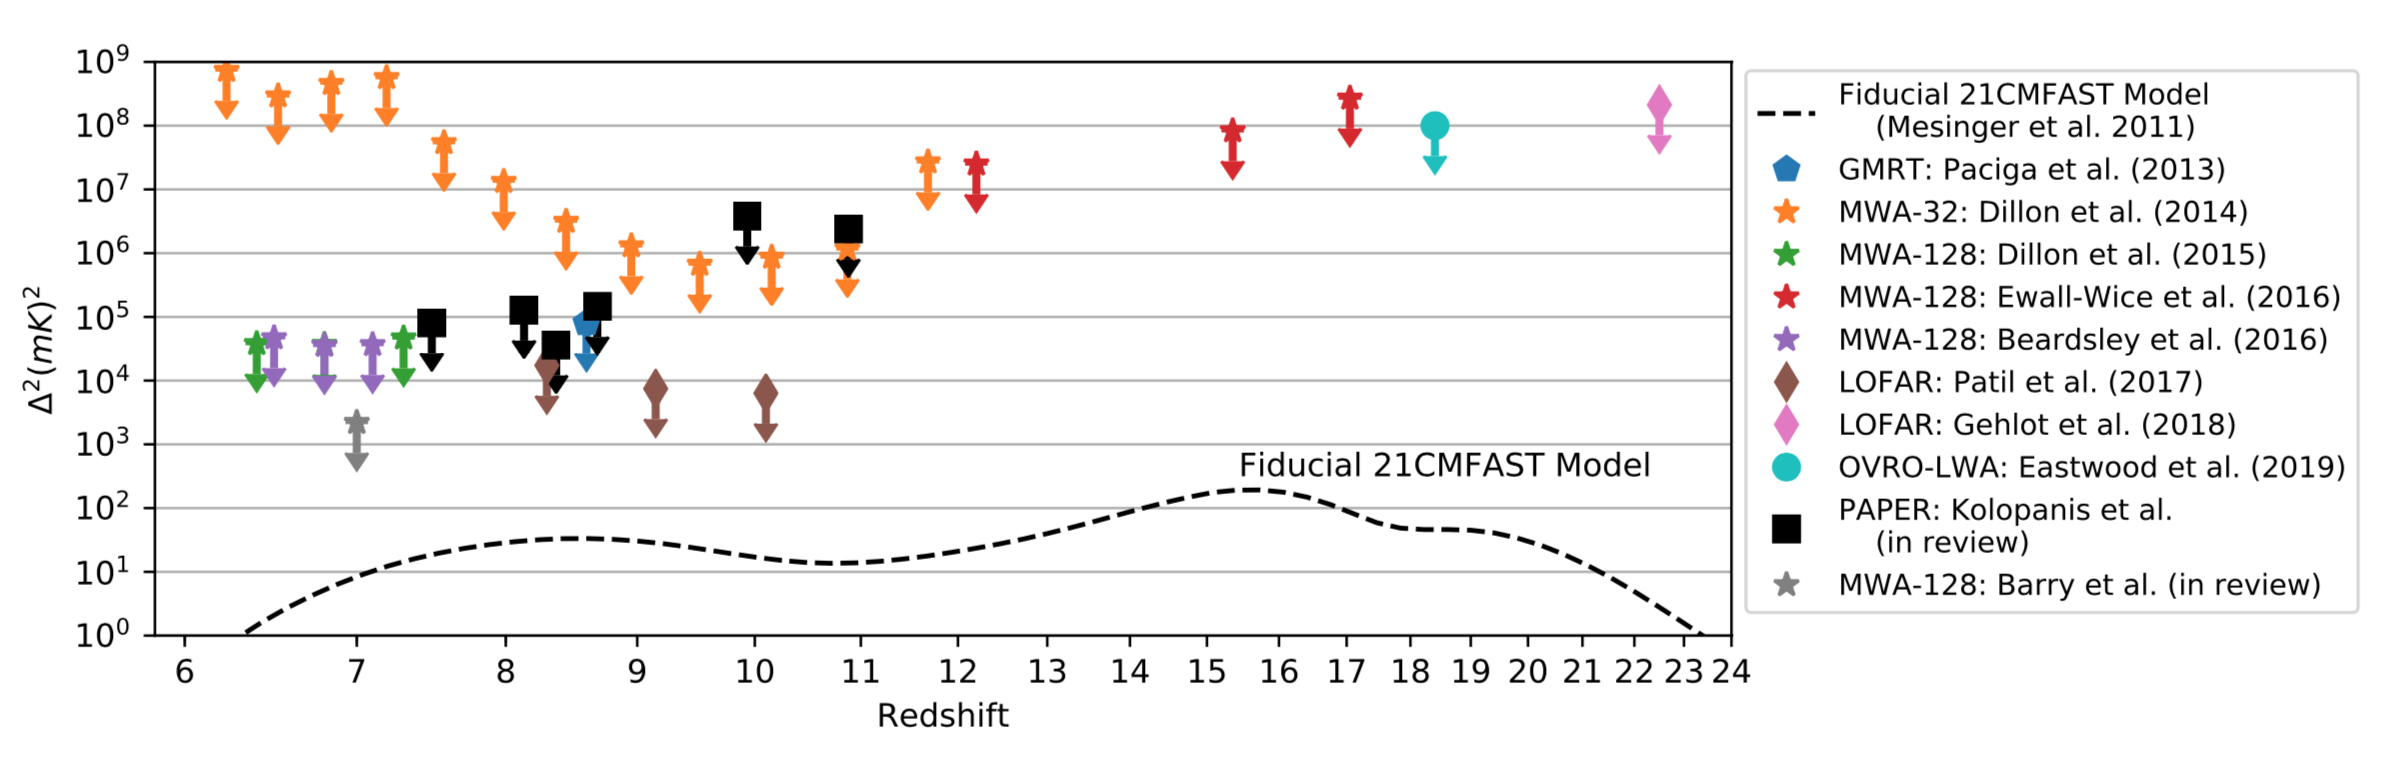
\includegraphics[width=1.\textwidth]{upper_limit.png}
	\caption[Upper Limits on Reionization]{A summary of the upper limits on the 21\,cm power spectrum across reionization. Plotted in the dashed line is a fiducial model of the 21\,cm power spectrum as simulated by \fastsim. Image taken from \cite{2019arXiv190708211L}}
	\label{fig:upper_limit}
\end{figure}
